\documentclass[12pt]{article}

\usepackage{alphabeta}
\usepackage[greek, english]{babel}
\usepackage[utf8]{inputenc}
\usepackage{geometry}
\usepackage{graphicx}
\usepackage{amsmath}
\usepackage{float}

\graphicspath{{images/}}
\geometry{left=.3in, right=.3in, top=0.6in, bottom=0.6in}
\renewcommand{\baselinestretch}{1.2}
\pagenumbering{gobble}
\let\endtitlepage\relax

\begin{document}
%% ------ Title
    \begin{titlepage}
    \vspace*{-0.6in}
    \begin{flushleft}
        
\includegraphics[scale=0.44]{images/logo.png}
        
        \vspace{1cm}
        \textbf{Ονοματεπώνυμο:} Ανδρέας Γουλέτας (3170031), Λούντζης Λάμπρος (3170095)\\ 
        \textbf{Εργασία:} Τεχνητή Νοημοσύνη\\
        \textbf{Ημερομηνία:} 7 Δεκεμβρίου 2020
        
    \end{flushleft}
    \vspace{0.2in}
\end{titlepage}
%% -------------------------------------------------------------------------------------
\section{Εισαγωγή}
\subsection{Περιγραφή Εργασίας}
Στο πρόβλημα \textbf{Bridge Crossing}, δοθέντος ενός συνόλου ατόμων, των χρόνων τους και μιας λάμπας, ζητείται να βρεθεί η καλύτερη δυνατή διάσχηση των ατόμων από την μια πλευρά της γέφυρας στην άλλη. Οι περιορισμοί που τίθενται είναι οι εξής:
\begin{itemize}
    \item μπορούν να διασχίζουν την γέφυρα ζευγάρια των δύο ατόμων κάθε φορά (ένας θα κρατάει την λάμπα), και ο χρόνος που λαμβάνεται υπόψη είναι αυτός του αργότερου,
    \item πρέπει να γυρίζει ένα άτομο με την λάμπα πίσω κάθε φορά.
\end{itemize}
Για την λύση του προβλήματος χρησιμοποιείται ο \textbf{αλγορίθμος αναζήτησης A*}. Eπίσης, θα παρουσίαζεται μια σύγκρισή των αποτελεσμάτων που παράγει με αυτά του \textbf{αλγορίθμου αναζήτησης BestFS.}
\subsection{Δομή παραδοτέου}
Αρχικά, στην Ενότητα 2 περιγράφεται η δομή των δεδομένων και δίνεται ένα παράδειγμα προς εκτέλεση. Στην Ενότητα 3 παρουσιάζεται ο \textbf{αλγόριθμος αναζήτησης A*} καθώς επίσης και τα αποτελέσματα που δίνει για το παράδειγμα της Ενότητας 2. Στην Ενότητα 4 παρουσιάζεται η \textbf{ευρετική συνάρτηση} που χρησιμοποιείται και αιτιολογείται γιατί είναι αποδεκτή. Τέλος, στην Ενότητα 5 δίνεται μια περιγραφή του \textbf{αλγορίθμου αναζήτησης BestFS}, τα αποτελέσματα για το παράδειγμα της Ενότητας 2 και παρουσιάζεται μια γραφική σύγκριση με τον αλγόριθμο αναζήτησης Α*.
%% -------------------------------------------------------------------------------------
\section{Δεδομένα}
Για την αναπαράσταση των δεδομένων έχουν επιλεχθεί αρχεία \textbf{CSV (Comma Separated Values)}. Η πρώτη γραμμή του αρχείου χρησιμοποιείται ως κεφαλίδα και αναφέρει ότι στην πρώτη στήλη θα πρέπει να υπάρχουν τα ονόματα των ατόμων (αλφαριθμητικά) ενώ στην δεύτερη στήλη οι χρόνοι διάσχισης τους (ακέραιοι αριθμοί μεγαλύτεροι του μηδενός).\\
Ενα ενδεικτικό dataset που χρησιμοποιείται και στην παρούσα εργασία είναι το dataset1.csv στον φάκελο dataset. Τα άτομα και οι χρόνοι που περιέχονται είναι οι εξής:
\begin{itemize}
    \item George - 1 sec
    \item Nick - 3 sec
    \item Maria - 6 sec
    \item Kostas - 8 sec
    \item Lampros - 12 sec
\end{itemize}
%% -------------------------------------------------------------------------------------
\section{Αλγόριθμος A*}
Για την εύρεση τελικής κατάστασης, δηλαδή μιας κατάστασης όπου όλα τα άτομα έχουν περάσει στην απέναντι πλεύρα της γέφυρας ή ο χρόνος έχει φτάσει ή υπερβεί το όριο που έχει δοθεί, χρησιμοποιείται ο \textbf{αλγόριθμος αναζήτησης A*}. Ο αλγόριθμος Α* αποτελεί έναν αλγόριθμο με πληροφόρηση, είναι βέτιστος και πλήρης. Για την αξιολόγηση των καταστάσεων χρησιμοποιείται η συνάρτηση
 \begin{equation*}
        f(n) = h(n) + g(n)
\end{equation*}\\
όπου n είναι ο κόμβος προς εξέταση, h είναι η ευρετική συνάρτηση που χρησιμοποείται και g είναι το κόστος της μετάβασης απο την κατάσταση-ρίζα στον κόμβο προς εξέταση.\\\\
\textbf{\underline{Παράδειγμα:}} Για είσοδο τα δεδομένα της Ενότητας 2, dataset1.csv, και όριο ίσο με 30sec, ο χρόνος που χρειάζονται τα άτομα να περάσουν στην απέναντι όχθη είναι 29sec
%% -------------------------------------------------------------------------------------
\section{Ευρετική Συνάρτηση}
Η \textbf{ευρετική συνάρτηση} που έχει υλοποιηθεί επιστρέφει ως αποτέλεσμα για κάθε κατάσταση το μέγιστο χρόνο από όλα τα άτομα που βρίσκονται στην όχθη εκκίνησης και δεν έχουν περάσει ακόμα. Είναι αποδεκτή διότι αποτελεί υποεκτίμηση της πραγματικότητας, αφού αναιρεί και τους δυο περιορισμόυ που έχουν τεθεί (δυο άτομα διασχίζουν την γέφυρα κάθε φορά και ένα άτομα γυρνάει πίσω).
%% -------------------------------------------------------------------------------------
\section{Σύγκριση με αλγόριθμο BestFS}
\subsection{Αλγόριθμος BesFS}
Ο \textbf{αλγόριθμος BestFS} χρησιμοποιεί πληροφόρηση, είναι άπληστος (επιλογή πάντα του κοντινότερου κόμβου με βάση την ευρετική), αλλά σε αντίθεση με τον A* δεν είναι πλήρης και βέλτιστος.  Για την αξιολόγηση των καταστάσεων χρησιμοποιείται η συνάρτηση
 \begin{equation*}
        f(n) = h(n)
\end{equation*}\\
όπου n είναι ο κόμβος προς εξέταση και h είναι η ευρετική συνάρτηση που χρησιμοποείται.\\\\
\textbf{\underline{Παράδειγμα:}} Για είσοδο τα δεδομένα της Ενότητας 2, dataset1.csv, και οριο ίσο με 30sec, δεν επιστρέφεται κάποια λύση. Αυτό οφείλεται στο γεγονός ότι είναι μη πλήρης. Αν αντιθέτως, δώσουμε όριο ίσο με μηδέν στο πρόγραμμά μας, ώστε να μην λαμβάνεται υπόψη, επιστρέφει λύση με χρόνο διάσχησης 46sec, τιμή μεγαλύτερη απο αυτή του αλγορίθμου A*. Παρατηρούμε, λοιπόν, οτι είναι και μη βέλτιστος.
\subsection{Σύγκριση}
Για την σύγκριση των αλγορίθμων Α* και BestFS χρησιμοποιούνται ώς είσοδο στο πρόγραμμα δέκα datasets (συμπεριλαμβανομένου και αυτού της Ενότητας 2) χωρίς κάποιο όριο, ώστε και οι δυο αλγόριθμοι να επιστρέφουν αποτελέσματα.\\
Από την γραφική παράσταση που ακολουθεί παρατηρείται ότι ο αλγόριθμος A* δίνει καλύτερους χρόνους διάσχισης από ότι ο BestFS. Αυτό οφείλεται στο γεγονός οτι ο συνυπολογισμός του κόστους απο τον κόμβο-ρίζα στον κόμβο προς εξέταση (συνάρτηση g) μαζί με το εκτιμώμενο κόστος της φθηνότερης διαδρομής από τον κόμβο n στον στόχο (συνάρτηση h) δίνει το εκτιμώμενο κόστος της φθινότερης λύσης μέσω του κόμβου n (συνάρτηση f).
\begin{figure}[H]
        \centering
        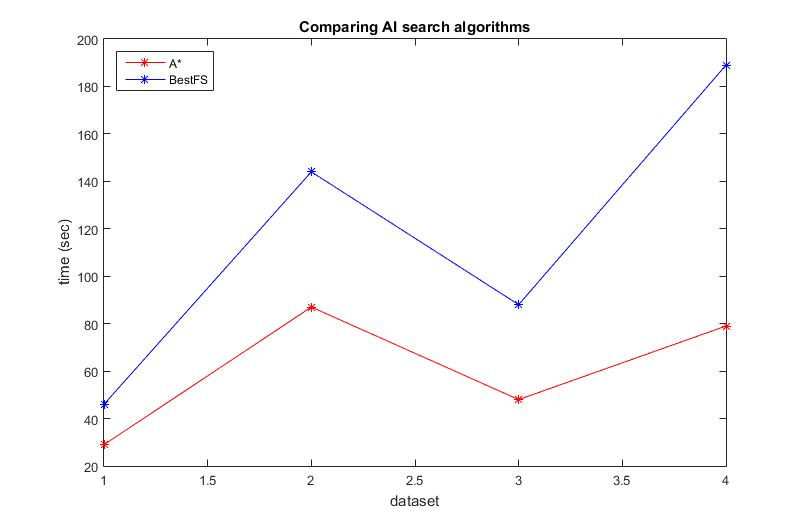
\includegraphics[scale=.6]{images/ai_res}
     \end{figure}
\end{document}
